\documentclass[border=10pt]{standalone}
\usepackage{tikz,graphicx,amsmath}
\usetikzlibrary{positioning,calc,arrows.meta,decorations.markings}

% ========== 颜色：四个阶段 ==========
\colorlet{myred}{red!80!black}
\colorlet{mygreen}{green!60!black}
\colorlet{myorange}{orange!70!red!60!black}
\colorlet{myblue}{blue!80!black}

\begin{document}
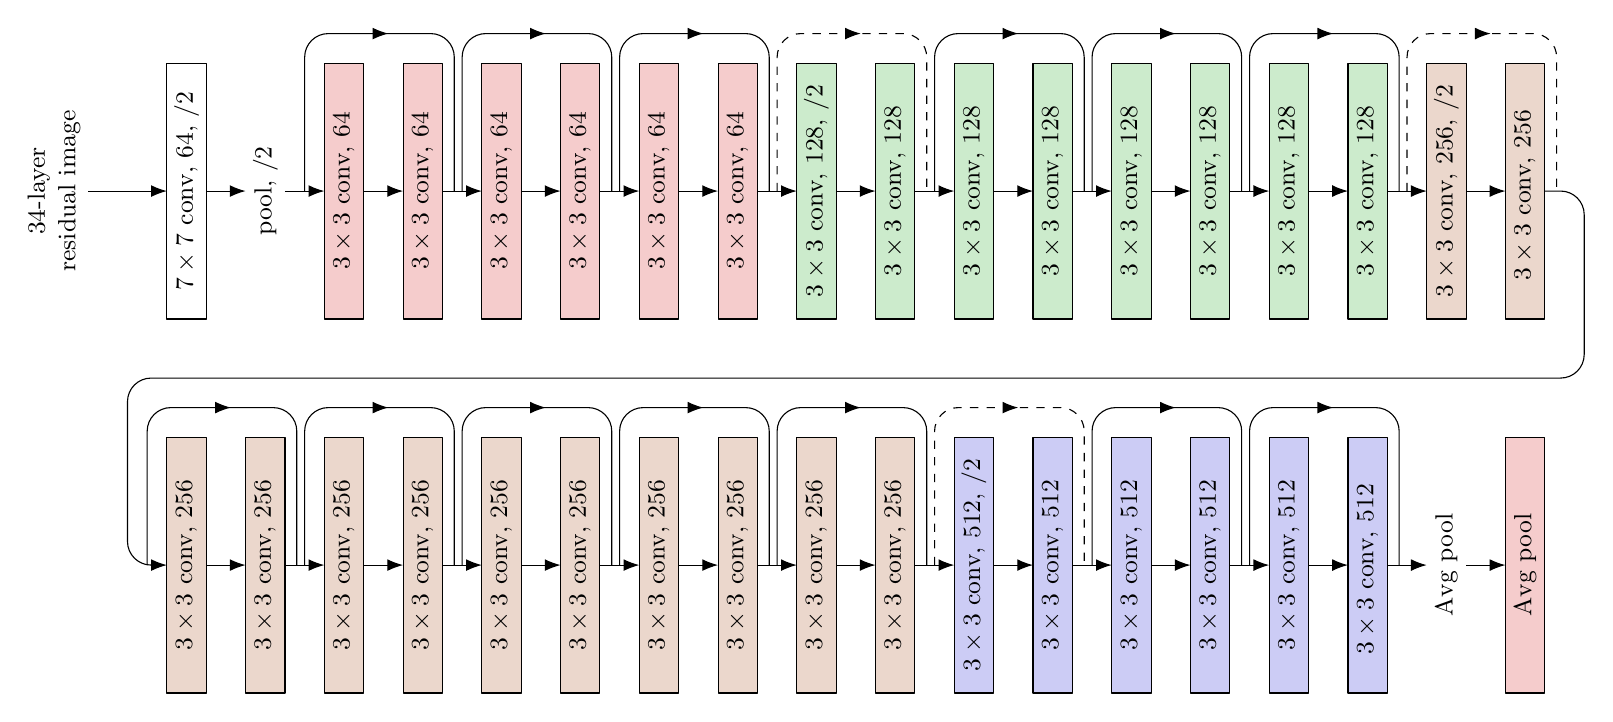
\begin{tikzpicture}[
    font=\small, line join=round,
    every node/.style={outer sep=0pt, inner sep=0pt},
    w/.style={minimum width=#1},
    h/.style={minimum height=#1},
    bar/.style={draw, w=.5cm, h=3.25cm},
    arr/.style={-{Latex[length=2mm, width=1.5mm]}},
    skip/.style={rounded corners=3mm, postaction={decorate},
                 decoration={markings, mark=at position 0.52 with {\arrow{Latex[length=2mm, width=1.5mm]}}}}
  ]

  % ========== 第一行：stem + 64 + 128 + 256 前半 ==========
  \node[bar, fill=white] (1) {\rotatebox{90}{$7\times7$ conv, $64$, /2}};
  \node[w=.5cm, h=3.25cm, right=.5cm of 1] (2) {\rotatebox{90}{pool, /2}};

  \foreach \n/\col/\txt [remember=\n as \prev (initially 2)] in {
    3/myred/{$3\times3$ conv, $64$},   4/myred/{$3\times3$ conv, $64$},
    5/myred/{$3\times3$ conv, $64$},   6/myred/{$3\times3$ conv, $64$},
    7/myred/{$3\times3$ conv, $64$},   8/myred/{$3\times3$ conv, $64$},
    9/mygreen/{$3\times3$ conv, $128$, /2}, 10/mygreen/{$3\times3$ conv, $128$},
    11/mygreen/{$3\times3$ conv, $128$}, 12/mygreen/{$3\times3$ conv, $128$},
    13/mygreen/{$3\times3$ conv, $128$}, 14/mygreen/{$3\times3$ conv, $128$},
    15/mygreen/{$3\times3$ conv, $128$}, 16/mygreen/{$3\times3$ conv, $128$},
    17/myorange/{$3\times3$ conv, $256$, /2}, 18/myorange/{$3\times3$ conv, $256$}
  } {\node[bar, fill=\col!20, right=.5cm of \prev] (\n) {\rotatebox{90}{\txt}};}

  % ========== 第二行：256 后半 + 512 + 池化 ==========
  \node[bar, fill=myorange!20, below=1.5cm of 1] (19) {\rotatebox{90}{$3\times3$ conv, $256$}};

  \foreach \n/\col/\txt [remember=\n as \prev (initially 19)] in {
    20/myorange/{$3\times3$ conv, $256$}, 21/myorange/{$3\times3$ conv, $256$},
    22/myorange/{$3\times3$ conv, $256$}, 23/myorange/{$3\times3$ conv, $256$},
    24/myorange/{$3\times3$ conv, $256$}, 25/myorange/{$3\times3$ conv, $256$},
    26/myorange/{$3\times3$ conv, $256$}, 27/myorange/{$3\times3$ conv, $256$},
    28/myorange/{$3\times3$ conv, $256$},
    29/myblue/{$3\times3$ conv, $512$, /2}, 30/myblue/{$3\times3$ conv, $512$},
    31/myblue/{$3\times3$ conv, $512$}, 32/myblue/{$3\times3$ conv, $512$},
    33/myblue/{$3\times3$ conv, $512$}, 34/myblue/{$3\times3$ conv, $512$}
  } {\node[bar, fill=\col!20, right=.5cm of \prev] (\n) {\rotatebox{90}{\txt}};}

  \node[w=.5cm, h=3.25cm, right=.5cm of 34] (35) {\rotatebox{90}{Avg pool}};
  \node[bar, fill=myred!20, right=.5cm of 35] (36) {\rotatebox{90}{Avg pool}};

  % ========== 主干箭头 ==========
  \draw[arr] ($(1.west)+(-1,0)$) --
    node[above, pos=0, align=center, rotate=90, yshift=1mm] {34-layer\\residual image} (1);
  \foreach \i [count=\j from 2] in {1,...,17} \draw[arr] (\i) -- (\j);
  \foreach \i [count=\j from 20] in {19,...,35} \draw[arr] (\i) -- (\j);

  % ========== 18 -> 19 回行连接 ==========
  \coordinate (u) at ($(1)!.5!(19)$);
  \draw[arr, rounded corners=3mm] (18.east) -- coordinate[pos=1] (v) ++(.5,0) -- (u-|v) -- ++(-18.5,0) |- (19);
  % ========== 残差跳跃：同阶段实线 ==========
  \foreach \i/\j/\k/\l in {2/3/4/5, 4/5/6/7, 6/7/8/9, 10/11/12/13, 12/13/14/15,
                           14/15/16/17, 20/21/22/23, 22/23/24/25, 24/25/26/27,
                           26/27/28/29, 30/31/32/33, 32/33/34/35}
    \draw[skip] ($(\i)!.5!(\j)$) -- ++(0,2) -| ($(\k)!.4!(\l)$);

  % ========== 残差跳跃：跨阶段虚线（下采样）==========
  \foreach \i/\j/\k/\l in {8/9/10/11, 28/29/30/31}
    \draw[skip, dashed] ($(\i)!.5!(\j)$) -- ++(0,2) -| ($(\k)!.4!(\l)$);

  \draw[skip] ($(19)+(-.5,0)$) -- ++(0,2) -| ($(20)!.4!(21)$);
  \draw[skip, dashed] ($(16)!.5!(17)$) -- ++(0,2) -| ($(18)+(.4,0)$);

\end{tikzpicture}
\end{document}